\section{量子统计力学}
\subsection{基本概念}
量子力学中本来就有随机, 即任给状态 $ \Psi(x) $, 观测它的物理量所得的结果是随机的. 现在我们在这层随机上再加一层随机, 我们让系统以概率 $ p_n $ 取状态 $ \Psi_n(x) $, 这就得到了量子力学中的系综, 我们称其为{\bf 混合态} (mixed state), 而称单个状态 $ \Psi(x) $ 为{\bf 纯态} (pure state).
\begin{remark}
    这里我们只允许混合态由至多可数个向量混合而成.
\end{remark}
定义混合态对应的{\bf 密度矩阵} (density matrix) 为
\[ \rho=\sum_n p_n| \Psi_n \rangle\langle \Psi_n |. \]
这里我们使用了物理中的记号, 用 $ | b \rangle\langle a | $ 表示算子 $ | \varphi \rangle\mapsto\langle a|\varphi \rangle\cdot| b \rangle $.
\begin{remark}
    密度矩阵其实不是矩阵, 是无穷维的``矩阵''. 我们可以仿照有限维的情况定义无穷维矩阵的一些运算, 但为了简洁, 我们不对这部分技术细节进行讨论.
\end{remark}
设 $ \{\Phi_\alpha\}_{\alpha=1}^{\infty} $ 是量子希尔伯特空间的一组基, $ A $ 为可观测量, 则对 $ \rho $ 测量 $ A $ 所得结果的期望为
\begin{align*}
    \langle A\rangle &=\sum_n p_n\langle \Psi_n |A| \Psi_n \rangle\\ 
    &=\sum_n p_n\langle \Psi_n |\left( \sum_\alpha| \Phi_\alpha \rangle\langle \Phi_\alpha | \right)A| \Psi_n \rangle\\ 
    &=\sum_n p_n\sum_\alpha\langle \Phi_\alpha | A| \Psi_n \rangle\langle \Psi_n |\Phi_\alpha\rangle\\ 
    &=\sum_\alpha \langle \Phi_\alpha | A\left( \sum_n p_n| \Psi_n \rangle\langle \Psi_n | \right)| \Phi_\alpha \rangle\\ 
    &= \mathrm{Tr}(A\rho),
\end{align*}
其中第二个等号是因为
\[ I=\sum_\alpha| \Phi_\alpha \rangle\langle \Phi_\alpha |. \]
\begin{example}
    纯态 $ \Psi $ 对应的密度矩阵为 $ \rho_{\mathrm{pure}}=| \Phi \rangle\langle \Phi | $.
\end{example}
\begin{proposition}
    对于纯态, 有 $ \rho_{\mathrm{pure}}^2=\rho_{\mathrm{pure}} $.
\end{proposition}
\begin{proposition}
    对于任意密度矩阵, 有 $ \mathrm{Tr}(\rho)=1 $.
\end{proposition}

\begin{proposition}
    密度矩阵随时间演化方式满足
    \[ \frac{\partial\rho}{\partial t}=\frac{1}{\mathrm{i}\hbar}[\hat{H},\rho]. \]
\end{proposition}
\begin{proof}
    使用薛定谔方程
    \[ \frac{\partial| \Psi_n \rangle}{\partial t}=\frac{1}{\mathrm{i}\hbar}\hat{H}| \Psi_n \rangle \]
    有
    \begin{align*}
        \frac{\partial\rho}{\partial t}&=\sum_n p_n\left( \frac{\partial| \Psi_n \rangle}{\partial t}\langle \Psi_n |+| \Psi_n \rangle\frac{\partial\langle \Psi_n |}{\partial t} \right)\\ 
        &=\sum_n \frac{p_n}{\mathrm{i}\hbar}\left( \hat{H}| \Psi_n \rangle\langle \Psi_n |-| \Psi_n \rangle\langle \Psi_n |\hat{H} \right)=\frac{1}{\mathrm{i}\hbar}[\hat{H},\rho].\qedhere
    \end{align*}
\end{proof}

假设哈密顿量 $ \hat{H} $ 拥有可数个特征向量 $ | E_n \rangle $, $ n=0,1,2,\dots $, 且它们构成一组正规正交基. 记 $ | E_n \rangle $ 对应的特征值为 $ E_n $, 称密度矩阵
\[ \rho_{\mathrm{canon}}:=\sum_n\frac{e^{-\beta E_n}}{Z}| E_n \rangle\langle E_n |, \]
对应的混合态为{\bf 正则分布} (canonical distribution), 其中 
\[ Z:=\sum_n e^{-\beta E_n}\sum_n\langle E_n |e^{-\beta \hat{H}}| E_n \rangle=\mathrm{Tr}\left( e^{-\beta \hat{H}} \right) \]
为配分函数. 由于
\[ \sum_n | E_n \rangle e^{-\beta E_n}\langle E_n |=e^{-\beta \hat{H}}, \]
我们可将正则分布的密度矩阵写为
\[ \rho_{\mathrm{canon}}=\frac{e^{-\beta\hat{H}}}{\mathrm{Tr}\left( e^{-\beta\hat{H}} \right)}. \]

类似经典统计力学的情况, 我们还可以定义密度矩阵 $ \rho $ 的熵为 
\[ S:=-k_B\mathrm{Tr}(\rho\log\rho). \]

\begin{example}[简谐振子]
    由章节 \ref{harmonic oscillator}, 简谐振子的哈密顿量的特征值为
    \[ E_n=\left( n+\frac{1}{2} \right)\hbar\omega. \]
    因此简谐振子的配分函数为
    \begin{align*}
        Z&=\sum_{n=0}^{\infty}e^{-\beta E_n}=\sum_{n=0}^{\infty}e^{-\beta\hbar\omega\left( n+\frac{1}{2} \right)}=e^{-\frac{\beta\hbar\omega}{2}}\sum_{n=0}^{\infty}\left( e^{-\beta\hbar\omega} \right)^n\\
        &=\frac{e^{-\frac{\beta\hbar\omega}{2}}}{1-e^{-\beta\hbar\omega}}=\frac{1}{e^{\frac{\beta\hbar\omega}{2}}-e^{-\frac{\beta\hbar\omega}{2}}}=\frac{1}{2\sinh\left( \frac{\beta\hbar\omega}{2} \right)}.
    \end{align*}
    利用经典正则系综的命题 \ref{internal energy} 可算得
    \begin{align*}
        \langle E\rangle &= -\frac{\partial\log Z}{\partial\beta}=\frac{\partial}{\partial\beta}\left[ \frac{\beta\hbar\omega}{2}+\log\left( 1-e^{-\beta\hbar\omega} \right) \right]\\ 
        &=\hbar\omega\left( \frac{1}{2}+\frac{1}{e^{\beta\hbar\omega}-1} \right),
    \end{align*}
    这说明平均激发层级为
    \[ \langle n\rangle=\frac{1}{e^{\beta\hbar\omega}-1}. \]
    
    又由命题 \ref{specific heat} 可得
    \[ c_v=\frac{\partial \langle E\rangle}{\partial T}=k_B\left( \frac{\hbar\omega}{k_B T} \right)^2\frac{e^{\beta\hbar\omega}}{\left( e^{\beta\hbar\omega}-1 \right)^2}. \]
    当温度很大时有
    \[ \lim_{T\to\infty}c_v=k_B, \]
    因此粒子的能量约为 $ k_BT/2 $, 这与能量均分定理的结论一致, 见例 \ref{ideal gas} (注意这里的简谐振子是一维的, 三维时粒子能量约为 $ 3k_BT/2 $).
\end{example}
\subsection{玻色子与费米子}
以下均假设粒子间无相互作用.
\begin{quantumaxiom}[全同粒子假设]
    内禀性质 (质量、电荷、自旋等) 完全相同的粒子叫做{\bf 全同粒子} (identical particles), 量子力学中的全同粒子是无法被区分的.
\end{quantumaxiom}

给定 $ N $ 个全同粒子, 记它们的波函数为 $ \Psi(r_1,\dots,r_N) $. 设 $ P=\{P_1,\dots,P_N\} $ 为 $ \{1,\dots,N\} $ 的一个排列, 当 $ P $ 为奇排列时定义 $ \sigma(P)=-1 $, 当 $ P $ 为偶排列时定义 $ \sigma(P)=1 $. 则
\begin{enumerate}
    \item[$ \bullet $] $ N $ 个全同玻色子的波函数是对称的, 即 $ \Psi(r_1,\dots,r_N)=\Psi(r_{P_1},\dots,r_{P_N}) $.
    \item[$ \bullet $] $ N $ 个全同费米子的波函数是反对称的, 即 $ \Psi(r_1,\dots,r_N)=\sigma(P)\Psi(r_{P_1},\dots,r_{P_N}) $.
\end{enumerate}

设 $ \Psi_k $ 为单个粒子的特征态, 则 $ N $ 个可区分粒子的特征态态形如
\[ \Psi_{\mathrm{dist}}(r_1,\dots,r_N)=\prod_{j=1}^N\psi_{k_j}(r_j), \]
其中 dist 为 distinguishable 的缩写.

对于不可取分的粒子, 交换任意两个粒子不会发生任何改变, 所以需要除以一个正则化系数. $ N $ 个全同玻色子的特征态形如
\[ \Psi_{\mathrm{boson}}(r_1,\dots,r_N)=C\sum_P\prod_{j=1}^N\psi_{k_j}(r_j), \]
其中 $ C $ 为正则化系数. 而 $ N $ 个全同费米子的特征态形如
\[ \Psi_{\mathrm{fermion}}(r_1,\dots,r_N)=\frac{1}{\sqrt{N!}}\sum_P\sigma(P)\prod_{j=1}^N\psi_{k_j}(r_j), \]
这个反对称化也可写成行列式的形式:
\[ \frac{1}{\sqrt{N!}}=\left| \begin{matrix}
    \psi_{k_1}(r_1) & \cdots & \psi_{k_1}(r_N)\\
    \vdots & \ddots & \vdots\\ 
    \psi_{k_N}(r_1) & \cdots & \psi_{k_N}(r_N)
\end{matrix} \right|, \]
这个行列式叫做 Slater 行列式.

\begin{example}[泡利不相容原理]
    两个全同玻色子的特征态形如
    \[ \frac{1}{\sqrt{2}}\left[ \psi_k(r_1)\psi_l(r_2)+\psi_k(r_2)\psi_l(r_1) \right]. \]
    两个全同费米子的特征态形如
    \[ \frac{1}{\sqrt{2}}\left[ \psi_k(r_1)\psi_l(r_2)-\psi_k(r_2)\psi_l(r_1) \right],\quad k\neq l. \]
    注意当 $ k=l $ 时, 有
    \[  \psi_k(r_1)\psi_k(r_2)-\psi_k(r_2)\psi_k(r_1)=0,  \]
    这说明两个费米子不能处于相同的特征态, 这就是{\bf 泡利不相容原理} (Pauli exclusion principle).
\end{example}

接下来, 我们要使用巨正则系综来处理玻色子和费米子. 我们将每个特征态视作一个系统, 特征态对应的系统之间相互独立, 且都可以与外界交换粒子. 因此每个特征态对应一个巨正则系综 $ \Xi_k $, 整体的对应的巨正则系综为 $ \bm\Xi=\prod_k\Xi_k $.

\subsubsection*{玻色-爱因斯坦统计}
对于玻色子, 我们可以以任意方式填充能级, 设特征态 $ \psi_k $ 对应的能量为 $ \varepsilon_k $, 固定化学势为 $ \mu $ (我们直接指出, 玻色子的化学势一定会小于粒子最小的特征值), 则
\[ \Xi^{\mathrm{boson}}_k=\sum_{n_k=0}^{\infty}e^{-\beta(\varepsilon_k-\mu)n_k}=\frac{1}{1-e^{-\beta(\varepsilon_k-\mu)}}. \]
因此玻色子的巨配分函数为
\[ \bm\Xi_{\mathrm{boson}}=\prod_k\frac{1}{1-e^{-\beta(\varepsilon_k-\mu)}}, \]
巨自由能为
\[ \bm\Phi_{\mathrm{boson}}=\sum_k\Phi_k^{\mathrm{boson}}=\sum_k k_BT\log\left( 1-e^{-\beta(\varepsilon_k-\mu)} \right). \]

对于每个特征态 $ \psi_k $, 我们可以计算期望粒子数
\[ \langle n_k\rangle=-\frac{\partial\Phi^{\mathrm{boson}}_k}{\partial\mu}=\frac{1}{e^{\beta(\varepsilon_k-\mu)}-1}. \]
我们称下述粒子数与能量的关系为{\bf 玻色-爱因斯坦分布} (Bose-Einstein distribution):
\[ \langle n\rangle_{\mathrm{BE}}:=\frac{1}{e^{\beta(\varepsilon-\mu)}-1}. \]

\subsubsection*{费米-狄拉克统计}
对于费米子, 只能有 $ n_k=0 $ 或 $ n_k=1 $, 因此固定化学势 $ \mu $ 后有
\[ \Xi^{\mathrm{fermion}}_k=\sum_{n_k=0}^{1}e^{-\beta(\varepsilon_k-\mu)n_k}=1+e^{-\beta(\varepsilon_k-\mu)}, \]
进而可求得费米子的巨配分函数
\[ \bm\Xi_{\mathrm{fermion}}=\prod_k\left( 1+e^{-\beta(\varepsilon_k-\mu)} \right). \]

可直接计算特征态 $ \psi_k $ 对应的期望粒子数:
\[ \langle n_k\rangle=\frac{\sum_{n_k=0}^{1}e^{-\beta(\varepsilon_k-\mu)n_k}}{\sum_{n_k=0}^{1}e^{-\beta(\varepsilon_k-\mu)n_k}}=\frac{1}{e^{\beta(\varepsilon_k-\mu)}+1}. \]
我们称下述粒子数与能量的关系为{\bf 费米-狄拉克分布} (Fermi-Dirac distribution):
\[ \langle n\rangle_{\mathrm{FD}}:=\frac{1}{e^{\beta(\varepsilon-\mu)}+1}. \]

\subsubsection*{麦克斯韦-玻尔兹曼统计}
现在我们要用经典统计力学去近似量子统计力学. 在经典统计力学中, 我们将粒子视为了可区分的, 而现在我们考虑的是全同粒子, 需要做修正:
\begin{align*}
    \Omega^{\mathrm{MB}}_N &= \frac{1}{N!}\Omega^{\mathrm{dist}}_N,\\
    Z^{\mathrm{MB}}_N &= \frac{1}{N!}Z^{\mathrm{dist}}_N.
\end{align*}
修正后所得的统计力学叫做{\bf 麦克斯韦-玻尔兹曼统计} (Maxwell-Boltzmann statistics).

对于正则系综, 单个粒子的经典正则配分函数为
\[ Z_1=\sum_ke^{-\beta\varepsilon_k}. \]
\begin{remark}
    这里的求和不是对能级求和, 而是对所有状态求和.
\end{remark}
多个 (可区分) 粒子的经典正则配分函数为
\[ Z^{\mathrm{dist}}_N=\sum_{k_1,\dots,k_N}e^{-\beta(\varepsilon_1+\dots+\varepsilon_{k_N})}=\prod_{j=1}^{N}\left( \sum_{k_j}e^{-\beta\varepsilon_{k_j}} \right)=(Z_1)^N. \]
\begin{remark}
    这里等式最右侧的上角标 $N$ 表示 $N$ 次幂.
\end{remark}
因此
\[ Z^{\mathrm{MB}}_N=\frac{1}{N!}(Z_1)^N. \]
进而对于巨正则系综有
\begin{align*}
    \bm\Xi^{\mathrm{MB}} &= \sum_N Z^{\mathrm{MB}}_Ne^{\beta\mu N}=\sum_N\frac{1}{N!}\left( \sum_{k}e^{-\beta\varepsilon_k} \right)^Ne^{\beta\mu N}\\ 
    &=\sum_N\frac{1}{N!}\left( \sum_k e^{-\beta(\varepsilon_k-\mu)} \right)^N=\exp\left( \sum_k e^{-\beta(\varepsilon_k-\mu)} \right)\\
    &=\prod_k\exp\left( e^{-\beta(\varepsilon_k-\mu)} \right).
\end{align*}
单个粒子的巨自由能为
\[ \Phi_i=k_BTe^{-\beta(\varepsilon_i-\mu)}, \]
整个系统的巨自由能为
\[ \bm\Phi^{\mathrm{MB}}=\sum_i \Phi_i, \]
下述粒子数期望与能量的关系叫做{\bf 玻尔兹曼分布} (Boltzmann distribution)
\[ \langle N\rangle_{\mathrm{MB}}:=-\frac{\partial\Phi}{\partial\mu}=e^{-\beta(\varepsilon-\mu)}. \]

综上, 粒子数期望与能量的关系总是满足
\[ \langle n\rangle=\frac{1}{e^{\beta(\varepsilon-\mu)}+c}, \]
其中玻色子取 $ c=-1 $, 费米子取 $ c=1 $, 麦克斯韦-玻尔兹曼统计取 $ c=0 $. 它们的函数图像如图 \ref{quantum statistical} 所示
\begin{figure}[htbp]
    \centering
    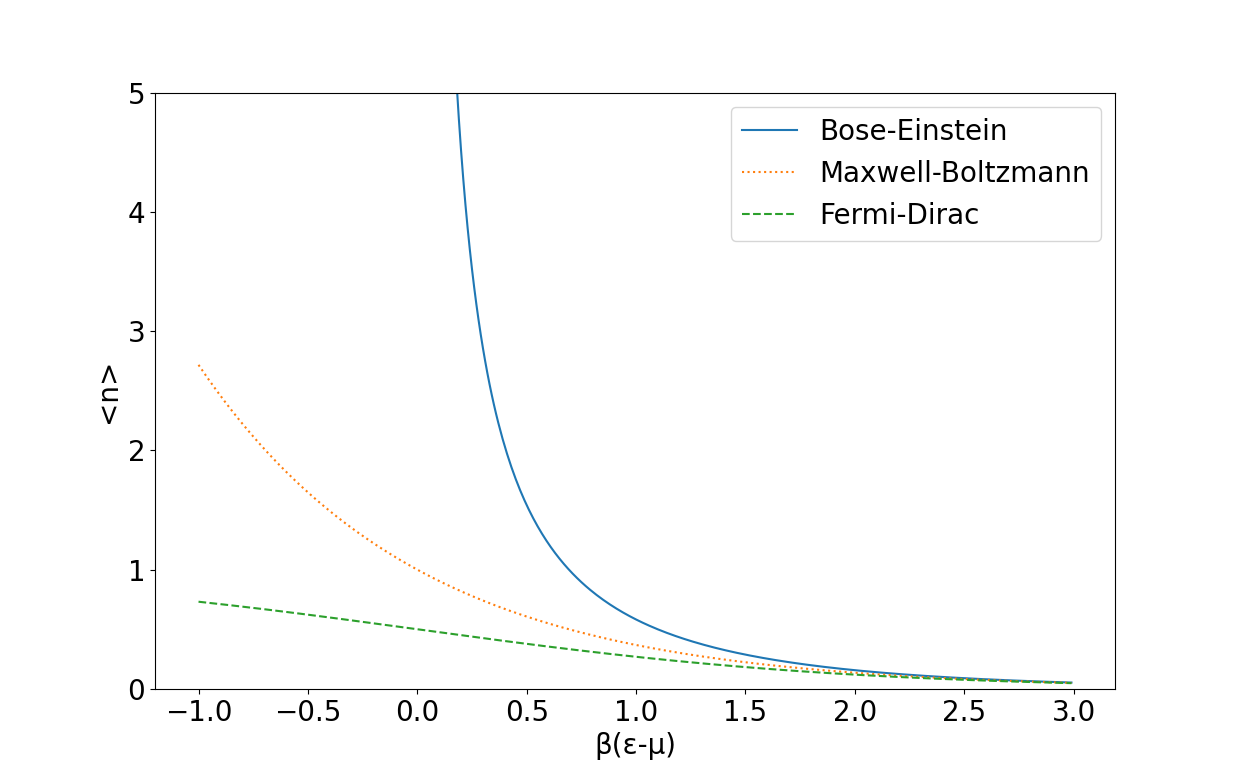
\includegraphics[width=\textwidth]{pic/quantum statistical.png}
    \caption{三种分布}
    \label{quantum statistical}
\end{figure}


\subsection{黑体辐射、凝聚态}
考虑边长为 $ L $ 的正方体盒子中的粒子, 在周期性边界条件下, 粒子的单位特征态为平面波
\[ \psi_k(r)=\left(\frac{1}{L}\right)^{\frac{3}{2}}e^{\mathrm{i}k\cdot r}, \]
其中
\[ k=\left(\begin{matrix}
    k_1\\k_2\\k_3
\end{matrix}\right)=\frac{2\pi}{L}\left(\begin{matrix}
    n_1\\n_2\\n_3
\end{matrix}\right),\quad n_1,n_2,n_3\in\mathbb{Z}. \]
记盒子的体积为 $ V=L^3 $, 则 $ k $ 所在的空间中单位体积对应约 $ V/(8\pi^3) $ 个特征态. 所有特征态对应的 $ k $ 形成了三维空间中的正方格点, 当 $ V $ 很大时, 格点非常密, 可以认为此时 $ k $ 所在的空间中特征态的密度为 $ V/(8\pi^3) $.
\subsubsection*{黑体辐射}
{\bf 黑体辐射}指的是处于平衡态的黑体发出的电磁辐射, 而{\bf 黑体}指的是可以完全吸收外来电磁辐射, 不进行反射和透射的物体. 电磁辐射就是电磁波, 或者从量子角度来看, 电磁辐射是由光子组成的. 光子的速度为光速 $ c $, 频率为 $ \omega=c|k| $, 另外由于电磁波有两个极化方向, 每个波向量 $ k $ 对应两个特征态.

固定温度 $ T $, 一小段频率 $ \mathrm{d}\omega $ 对应的特征态数量 $ g(\omega)\,\mathrm{d}\omega $ 为
\[ g(\omega)\,\mathrm{d}\omega=(4\pi k^2)\left( \frac{\mathrm{d}|k|}{\mathrm{d}\omega}\,\mathrm{d}\omega \right)\left( \frac{2V}{(2\pi)^3} \right), \]
其中等式右侧的第一项是半径为 $ k $ 的球面表面积, 第二项是频率变化 $ \mathrm{d}\omega $ 后半径为 $ k $ 的球面随之变化产生的球壳厚度, 第三项是特征态的密度. 带入 
\[ \frac{\mathrm{d}|k|}{\mathrm{d}\omega}=\frac{1}{c} \] 
可知单位频率对应的特征态数量为
\[ g(\omega)=\frac{V\omega^2}{\pi^2c^3}. \]

光子是玻色子, 化学势为 $ 0 $, 能量和频率的关系为 $ \varepsilon=\hbar\omega $. 根据前文中的结论可得频率 $\omega$ 对应的特征态的光子数 $n_\omega$ 满足
\[ \langle n_\omega\rangle=\frac{1}{e^{\hbar\omega/(k_BT)}-1}, \]
因此每 $ \mathrm{d}\omega $ 频率对应的光子数 $n$ 满足
\[ \langle n\rangle\,\mathrm{d}\omega=\frac{g(\omega)}{e^{\hbar\omega/(k_BT)}-1}\,\mathrm{d}\omega. \]
进一步地, 设 $ u(\omega) $ 为每单位体积的光子能量, 则每 $\mathrm{d}\omega$ 频率对应的能量为
\begin{align*}
    Vu(\omega)\,\mathrm{d}\omega &= \frac{\hbar\omega g(\omega)}{e^{\hbar\omega/(k_BT)}-1}\,\mathrm{d}\omega\\ 
    &=\frac{V\hbar}{\pi^2c^3}\frac{\omega^3\,\mathrm{d}\omega}{e^{\hbar\omega/(k_BT)}-1},
\end{align*}
这就是{\bf 普朗克黑体辐射定律} (Planck's law). 当频率很低时, 作近似 
\[ e^{\hbar\omega/(k_BT)}-1\approx\frac{\hbar\omega}{k_BT} \]
可以得到{\bf 瑞利-金斯定律} (Rayleigh-Jeans law)
\[ u(\omega)\,\mathrm{d}\omega= \left(\frac{k_BT}{\pi^2c^3}\right)\omega^2\,\mathrm{d}\omega. \]

\subsubsection*{凝聚态}
若盒子中有大量质量为 $ m $ 的全同玻色子, 由于 $ p=\hbar k $, 动量空间中特征态个数的密度为 $ V/(2\pi\hbar)^3 $. 单个粒子的能量为 $ \varepsilon=p^2/(2m) $, 且
\[ \frac{\mathrm{d}\varepsilon}{\mathrm{d}|p|}=\frac{|p|}{m}=\sqrt{\frac{2\varepsilon}{m}}, \]
因此每 $ \mathrm{d}\varepsilon $ 能量对应的特征态的数量为
\[ g(\varepsilon)\,\mathrm{d}\varepsilon=(4\pi p^2)\left( \frac{\mathrm{d}|p|}{\mathrm{d}\varepsilon}\,\mathrm{d}\varepsilon \right)\left( \frac{V}{(2\pi\hbar)^3} \right)=\frac{Vm^{\frac{3}{2}}}{\sqrt{2}\pi^2\hbar^3}\sqrt{\varepsilon}\,\mathrm{d}\varepsilon. \]

类似于一份电磁波能量 ($ \hbar\omega $) 对应一个光子, 设化学势为 $ \mu $, 根据玻色-爱因斯坦分布可知此时``总粒子数''为
\[ N(\mu)=\int_{0}^{\infty}\frac{g(\varepsilon)}{e^{(\varepsilon-\mu)/(k_BT)}-1}\,\mathrm{d}\varepsilon. \]
玻色子的化学势一定小于粒子最低的能量, 因此总是有 $ \mu<0 $. 我们可以通过提升化学势来使粒子被分配到每一个特征态中, 其极限状态为 $ \mu=0 $, 此时 $ N $ 达到最大值
\begin{align*}
    N_{\mathrm{max}} &= \int_0^\infty\frac{g(\varepsilon)}{e^{\varepsilon/(k_BT)}-1}\,\mathrm{d}\varepsilon\\ 
    &= \frac{Vm^{\frac{3}{2}}}{\sqrt{2}\pi^2\hbar^3}\int_{o}^{\infty}\frac{\sqrt{\varepsilon}}{e^{\varepsilon/(k_BT)}-1}\,\mathrm{d}\varepsilon\\ 
    &=V\left( \frac{\sqrt{2\pi mk_BT}}{h} \right)^3\frac{2}{\sqrt{\pi}}\int_{\sqrt{z}}^{e^z-1}\,\mathrm{d}z\\ 
    &=\left( \frac{V}{\lambda^3} \right)\zeta\left( \frac{3}{2} \right).
\end{align*}
因此盒子中所允许的最大``粒子密度''为
\[ \frac{N_{\mathrm{max}}}{V}=\frac{\zeta\left( \frac{3}{2} \right)}{\lambda^3}\approx\frac{2.612}{\lambda^3}. \]
假设``粒子数''已达最大值, 但我们还是继续往盒子中塞进新的粒子, 那么多出来的粒子都会被迫处于基态 (能量最低的特征态), 如果我们再继续加入大量的粒子, 那么大部分粒子都会处于基态, 这就是{\bf 玻色-爱因斯坦凝聚态} (Bose-Einstein condensation). 由全同粒子假设知, 这些处于基态的粒子们不可被区分, 换句话说, 它们的行为``整齐划一'', 进而诱发了超流、超导等现象.

另外, 我们也可以固定 $ N $ 和 $ V $, 不断降低温度, 当温度低至
\[ \frac{h^2}{2\pi mk_B}\left( \frac{N}{V\zeta\left( \frac{3}{2} \right)} \right)^{\frac{2}{3}} \]
时也会出现玻色-爱因斯坦凝聚态.